
\documentclass[a4paper,kul]{kulakarticle} %options: kul or kulak (default)

\usepackage[utf8]{inputenc}
\usepackage[dutch]{babel}
\usepackage{graphicx}
\usepackage{hyperref}
\usepackage{caption}
\usepackage{subcaption}

\date{31/05/2019}
\address{
  Faculteit Industriële Ingenieurswetenschappen \\
  Projectlab bachelor elektronica-ICT \\
  J. Lannoo, L. Espeel}
\title{Verslag E-ink room reservation display}
\author{Baptiste Pattyn\and Michel Dequick \and Stijn Declerck \and Ine Vanderhaeghe}


\begin{document}

\maketitle

\begin{center}
	\centering
	\vspace*{\fill}
	\huge
	\textbf{E-ink room reservation display}
	\vspace*{\fill}
\end{center}

\newpage

\section{Inhoud}

\tableofcontents

\newpage

\section{Probleemstelling}
{\scriptsize Geschreven door Ine}
\newline

De bedoeling van dit project is om een display te maken voor klaslokalen, dat dynamisch kan veranderen per uur. 

Op het scherm moeten verschillende zaken komen: het nummer van het klaslokaal, de datum, op welke uren het lokaal bezet is op een bepaalde dag, welk vak op dit moment gegeven wordt en de docent van dit vak.
\newline

Er zijn verschillende zaken waar rekening mee gehouden moet worden om dit te realiseren:

Er moet een E-ink display geïmplementeerd worden. Hierbij wordt bekeken als er burn-in of ghosting kan optreden. Ook wordt rekening gehouden met de grootte van de memory in de display.

Er moet een databank opgezet worden waar alle data van de lokalen in opgeslagen is. Deze databank is bereikbaar via wifi.

Er moet een connectie gemaakt worden via een wifi module van de databank naar de display.
\newline

Een E-ink display krijgt hier de voorkeur, omdat dit het meest energiezuinig is. Dit is zo omdat de display enkel voeding nodig heeft om het scherm te veranderen. Het scherm moet maar om het uur aangepast worden, dus alle tijd daartussen heeft een E-ink display geen voeding nodig.
Een ander voordeel van een E-ink display is dat het geen licht uitzendt, maar het reflecteert licht zoals een blad papier. Hierdoor is het gemakkelijker leesbaar, ook als er in de omgeving veel licht is. 
\newline

De eenvoudigste E-ink display is de "two pigment ink system". Dit bestaat uit kleine gebieden die dipolen zijn (deze worden gebruikt als de pixels van de afbeelding). De positieve kant van de gebieden bestaat uit wit pigment, de negatieve kant is zwart pigment. Deze gebieden bevinden zich in een bubbel van olie zodat ze gemakkelijk kunnen omdraaien, en zitten tussen transparante elektrode lagen. Wanneer nu op die elektrodelagen een spanning wordt gezet, kan bepaald worden welke delen van het scherm zwart zijn, en welke wit. Op die manier kan een zwart-wit afbeelding op de display geprogrammeerd worden. (zie afbeelding \ref{fig:2psystem} ).

\begin{figure}[h]
	\centering
	\begin{subfigure}{.5\textwidth}
		\centering
		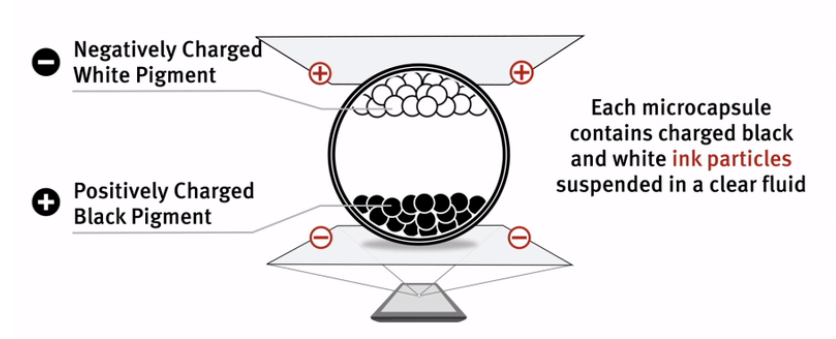
\includegraphics[width=0.95\textwidth]{Two_pigment_ink_system1}
		\label{fig:sub2psystem}
	\end{subfigure}%
	\begin{subfigure}{.5\textwidth}
		\centering
		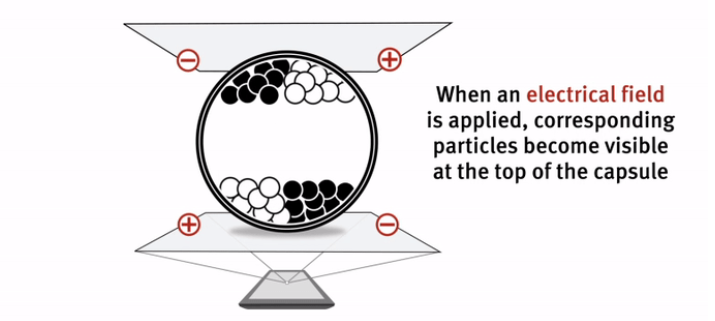
\includegraphics[width=0.95\textwidth]{Two_pigment_ink_system2}
		\label{fig:sub2psystem2}
	\end{subfigure}
	\caption{two pigment ink system}
	\label{fig:2psystem}
\end{figure}

Er bestaat ook een "Three pigment ink system". Dit werkt op ongeveer dezelfde manier als two pigment ink system (zie afbeelding \ref{fig:3psystem} ). Hier is het witte pigment negatief geladen en het rode pigment is positief geladen. Om het zwarte pigment aan de oppervlakte te brengen, moet er een gesplitste lading aangebracht worden.

\begin{figure}[h]
	\centering
	\begin{subfigure}{.5\textwidth}
		\centering
		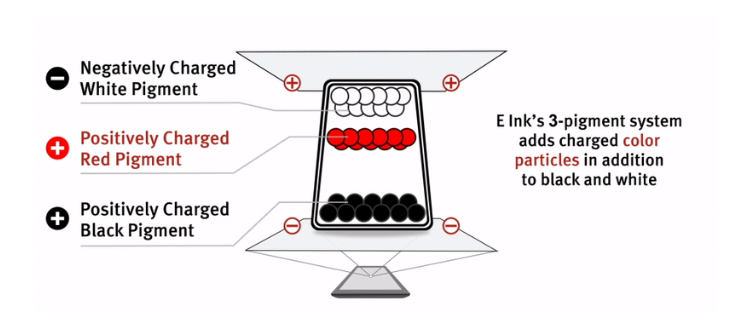
\includegraphics[width=0.95\textwidth]{three_pigment_ink_system1}
		\label{fig:sub3psystem}
	\end{subfigure}%
	\begin{subfigure}{.5\textwidth}
		\centering
		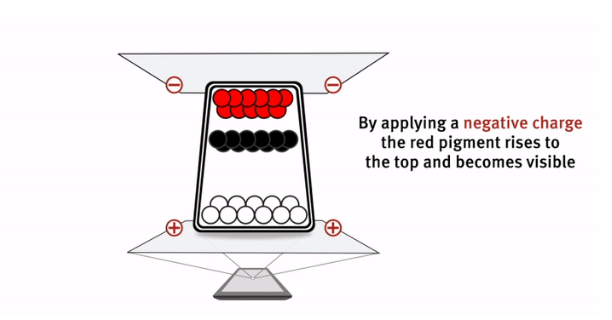
\includegraphics[width=0.95\textwidth]{three_pigment_ink_system2}
		\label{fig:sub3psystem2}
	\end{subfigure}
	\caption{three pigment ink system}
	\label{fig:3psystem}
\end{figure}

De E-ink display die in dit project gebruikt wordt, gebruikt het three pigment ink system. Op deze manier kan op een overzichtelijke manier op een tijdslijn aangeduid worden op welke uren het lokaal bezet is.
\newline

Daarnaast bestaat er ook een "Advanced color ePaper". Hierbij kunnen nog meer kleuren op het scherm afgebeeld worden. (zie afbeelding \ref{fig:ACeP} ). Dit wordt in dit project niet gebruikt. Dit systeem gebruikt 4 kleuren: cyaan, magenta, geel en wit.  \newline

\begin{figure}[h]
	\centering
	\begin{subfigure}{.5\textwidth}
		\centering
		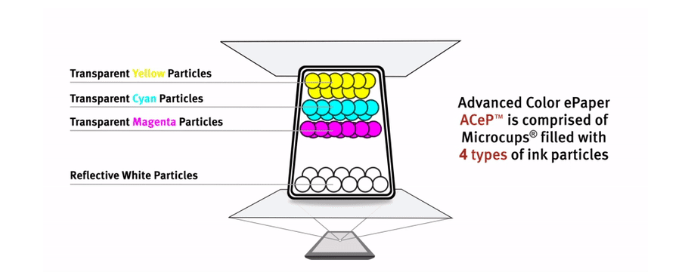
\includegraphics[width=0.95\textwidth]{ACeP1}
		\label{fig:subACeP}
	\end{subfigure}%
	\begin{subfigure}{.5\textwidth}
		\centering
		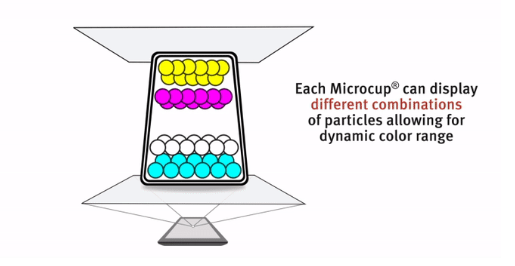
\includegraphics[width=0.95\textwidth]{ACeP2}
		\label{fig:subACeP2}
	\end{subfigure}
	\caption{Advanced color ePaper}
	\label{fig:ACeP}
\end{figure}

bron figuren: \cite{E-ink}.

bron werking ACeP: \cite{ACeP}.
\newline
\newline
Dit is het materiaal dat gebruikt werd:
\newline
Mbed FRDM-K64F

met application shield en click shield
\newline
ESP-WROOM-02 click met ESP8266EX wifi bord

Datasheet ESP-WROOM-02: \cite{ESP-WROOM-02}

Datasheet ESP8266EX: \cite{ESP8266EX}
\newline
Eink click, small and big display

\newpage

\section{Aanpak}
{\scriptsize Geschreven door Ine}
\newline

Eerst hebben we alle deelopdrachten op een rijtje gezet en een planning gemaakt. Daarbij maakten we ook een taakverdeling op. 
\newline
\newline
Dit zijn de grootste taken:
\newline
\newline
Een library maken voor de display – Michel
\newline
Eerst werd er bekeken hoe we een afbeelding op de display konden krijgen. Op het internet vonden we een voorbeeld van een E-ink display die gemaakt was met een Arduino. Wij maken gebruik van een mbed, dus we moesten de code aanpassen. 
Als eerste hebben we geprobeerd om een afbeelding op de display te zetten én om een afbeelding die er op staat uit te wissen.
Daarna maakten we een ontwerp van wat we allemaal op het scherm wilden hebben en waar juist. We hebben dan ook geprobeerd om dit op de display te krijgen.
\newline
\newline
Een database opstellen met een wifi access point – Baptiste
\newline
We hebben een database opgesteld op een Raspberry Pi. Daar werd ook een wifi access point op geïmplementeerd zodat de display met de databank kan communiceren.
Eens de databank opgevuld was kon getest worden als de data in een tabel per lokaal gezet kon worden.
\newline
\newline
Wifi connectiviteit en JSON parser maken – Stijn
\newline
Het is belangrijk om via wifi te kunnen communiceren tussen de E-ink display en de databank. Hiervoor moesten we onderzoeken hoe een HTTP GET request werkt en hoe we het zelf konden implementeren in onze toepassing.
\newline
Er moet ook een manier gevonden worden om de data te versturen. Hiervoor werd een JSON parser gemaakt.
\newline
\newline
Er waren ook enkele kleinere taken:
\newline
\newline
De databank invullen – Ine
\newline
De databank werd opgevuld met fictieve data over de lokaalbezetting zodat we een proof of concept konden maken om voor te stellen op de presentatie van ons project.
\newline
\newline
Het verslag en de powerpointpresentatie opstarten – Ine 
\newline
Om het verslag te maken heeft iedereen het deel waar hij zelf het meest aan gewerkt heeft aangevuld. 
\newline

In figuur \ref{fig:aanpak} is te zien hoe de verschillende delen aan elkaar gelinkt zijn.

\begin{figure}[h]
	\centering
	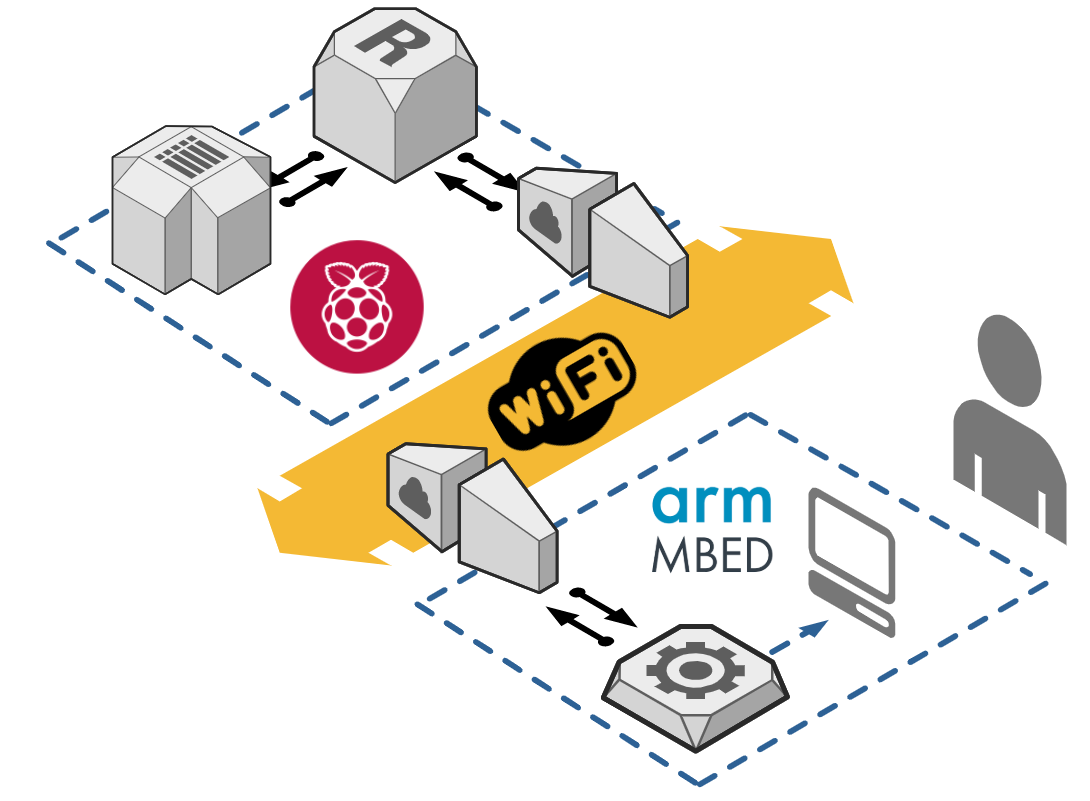
\includegraphics[width=0.75\textwidth]{Solution_workflow}
	\caption{aanpak}
	\label{fig:aanpak}
\end{figure}

\newpage

\section{Implementatie}
\subsection{Database en Wifi Access Point} 
{\scriptsize Geschreven door Baptiste}
\newline

Voor het opslaan van de gegevens is er een database opgezet op een Raspberry Pi model B+ door gebruik te maken van phpMyAdmin. Hier draait een SQL server op waarin alle gegevens voor de komende events van verschillende lokalen kunnen opgeslagen worden. Verder zijn alle gegevens van de courses er ook opgeslagen en de algemene info van de rooms. Om ervoor te zorgen dat onze MBED toegang kan krijgen tot deze database hebben we een Wifi Access Point (WAP) op de Raspberry Pi gezet, waarmee de MBED zich kan verbinden via een ESP8266 Wifi chip. Het opvragen van de gegevens door de mbed gebeurt via een GET request op de HTTP poort van de Raspberry Pi (poort 80).
 
\subsubsection{Database}
Deze database genaamd roomdb bestaat uit 3 verschillende tables: courses, events en rooms. De structuur van de database en de relaties tussen de verschillende tables staat afgebeeld in figuur \ref{fig:dbstruct}. Op de Raspberry Pi staan verschillende PHP files die ervoor zorgen dat de webserver kan verbinden met de database. Een belangrijke file hierbij is dbConnect.php (zie figuur \ref{fig:dbconnect}), in deze file staan de gegevens die nodig zijn om te kunnen verbinden met de database. In deze  file declareren we verschillende variabelen: \verb|$host|, \verb|$user|, \verb|$password|en \verb|$databse|. Deze worden dan gebruikt in een \verb|mysqli_connect()| commando om een verbinding op te zetten met de databse. Hierna wordt er nog een controle gedaan om te kijken of de verbinding tot stand is gekomen, indien dit niet het geval is wordt er een error gegenereerd. Deze code is enkel bedoeld voor tijdens het opzetten van de webserver en de database en dient verwijderd te worden indien de code definitief in gebruik wordt genomen. Als \verb|$host| wordt het local host adres 127.0.0.1 gebruikt omdat de database zich op de Raspberry Pi zelf bevindt. De \verb|$user| en het \verb|$password| zijn specifiek voor elke database en hangen af van welke user ingesteld werden op de SQL server. 
\begin{figure}[h]
	\begin{verbatim}
	<?php
	$host = "127.0.0.1";
	$user = "root";
	$password = "password" ;
	$database = "roomdb";
	$conn = mysqli_connect($host, $user, $password, $database);
	// delete when ready to launch
	if(!$conn){
	die("Connection failed: " . $conn ->connect_error);
	}
	?>
	\end{verbatim}
	\caption{dbConnect.php}
	\label{fig:dbconnect}
\end{figure}
\begin{figure}[h]
	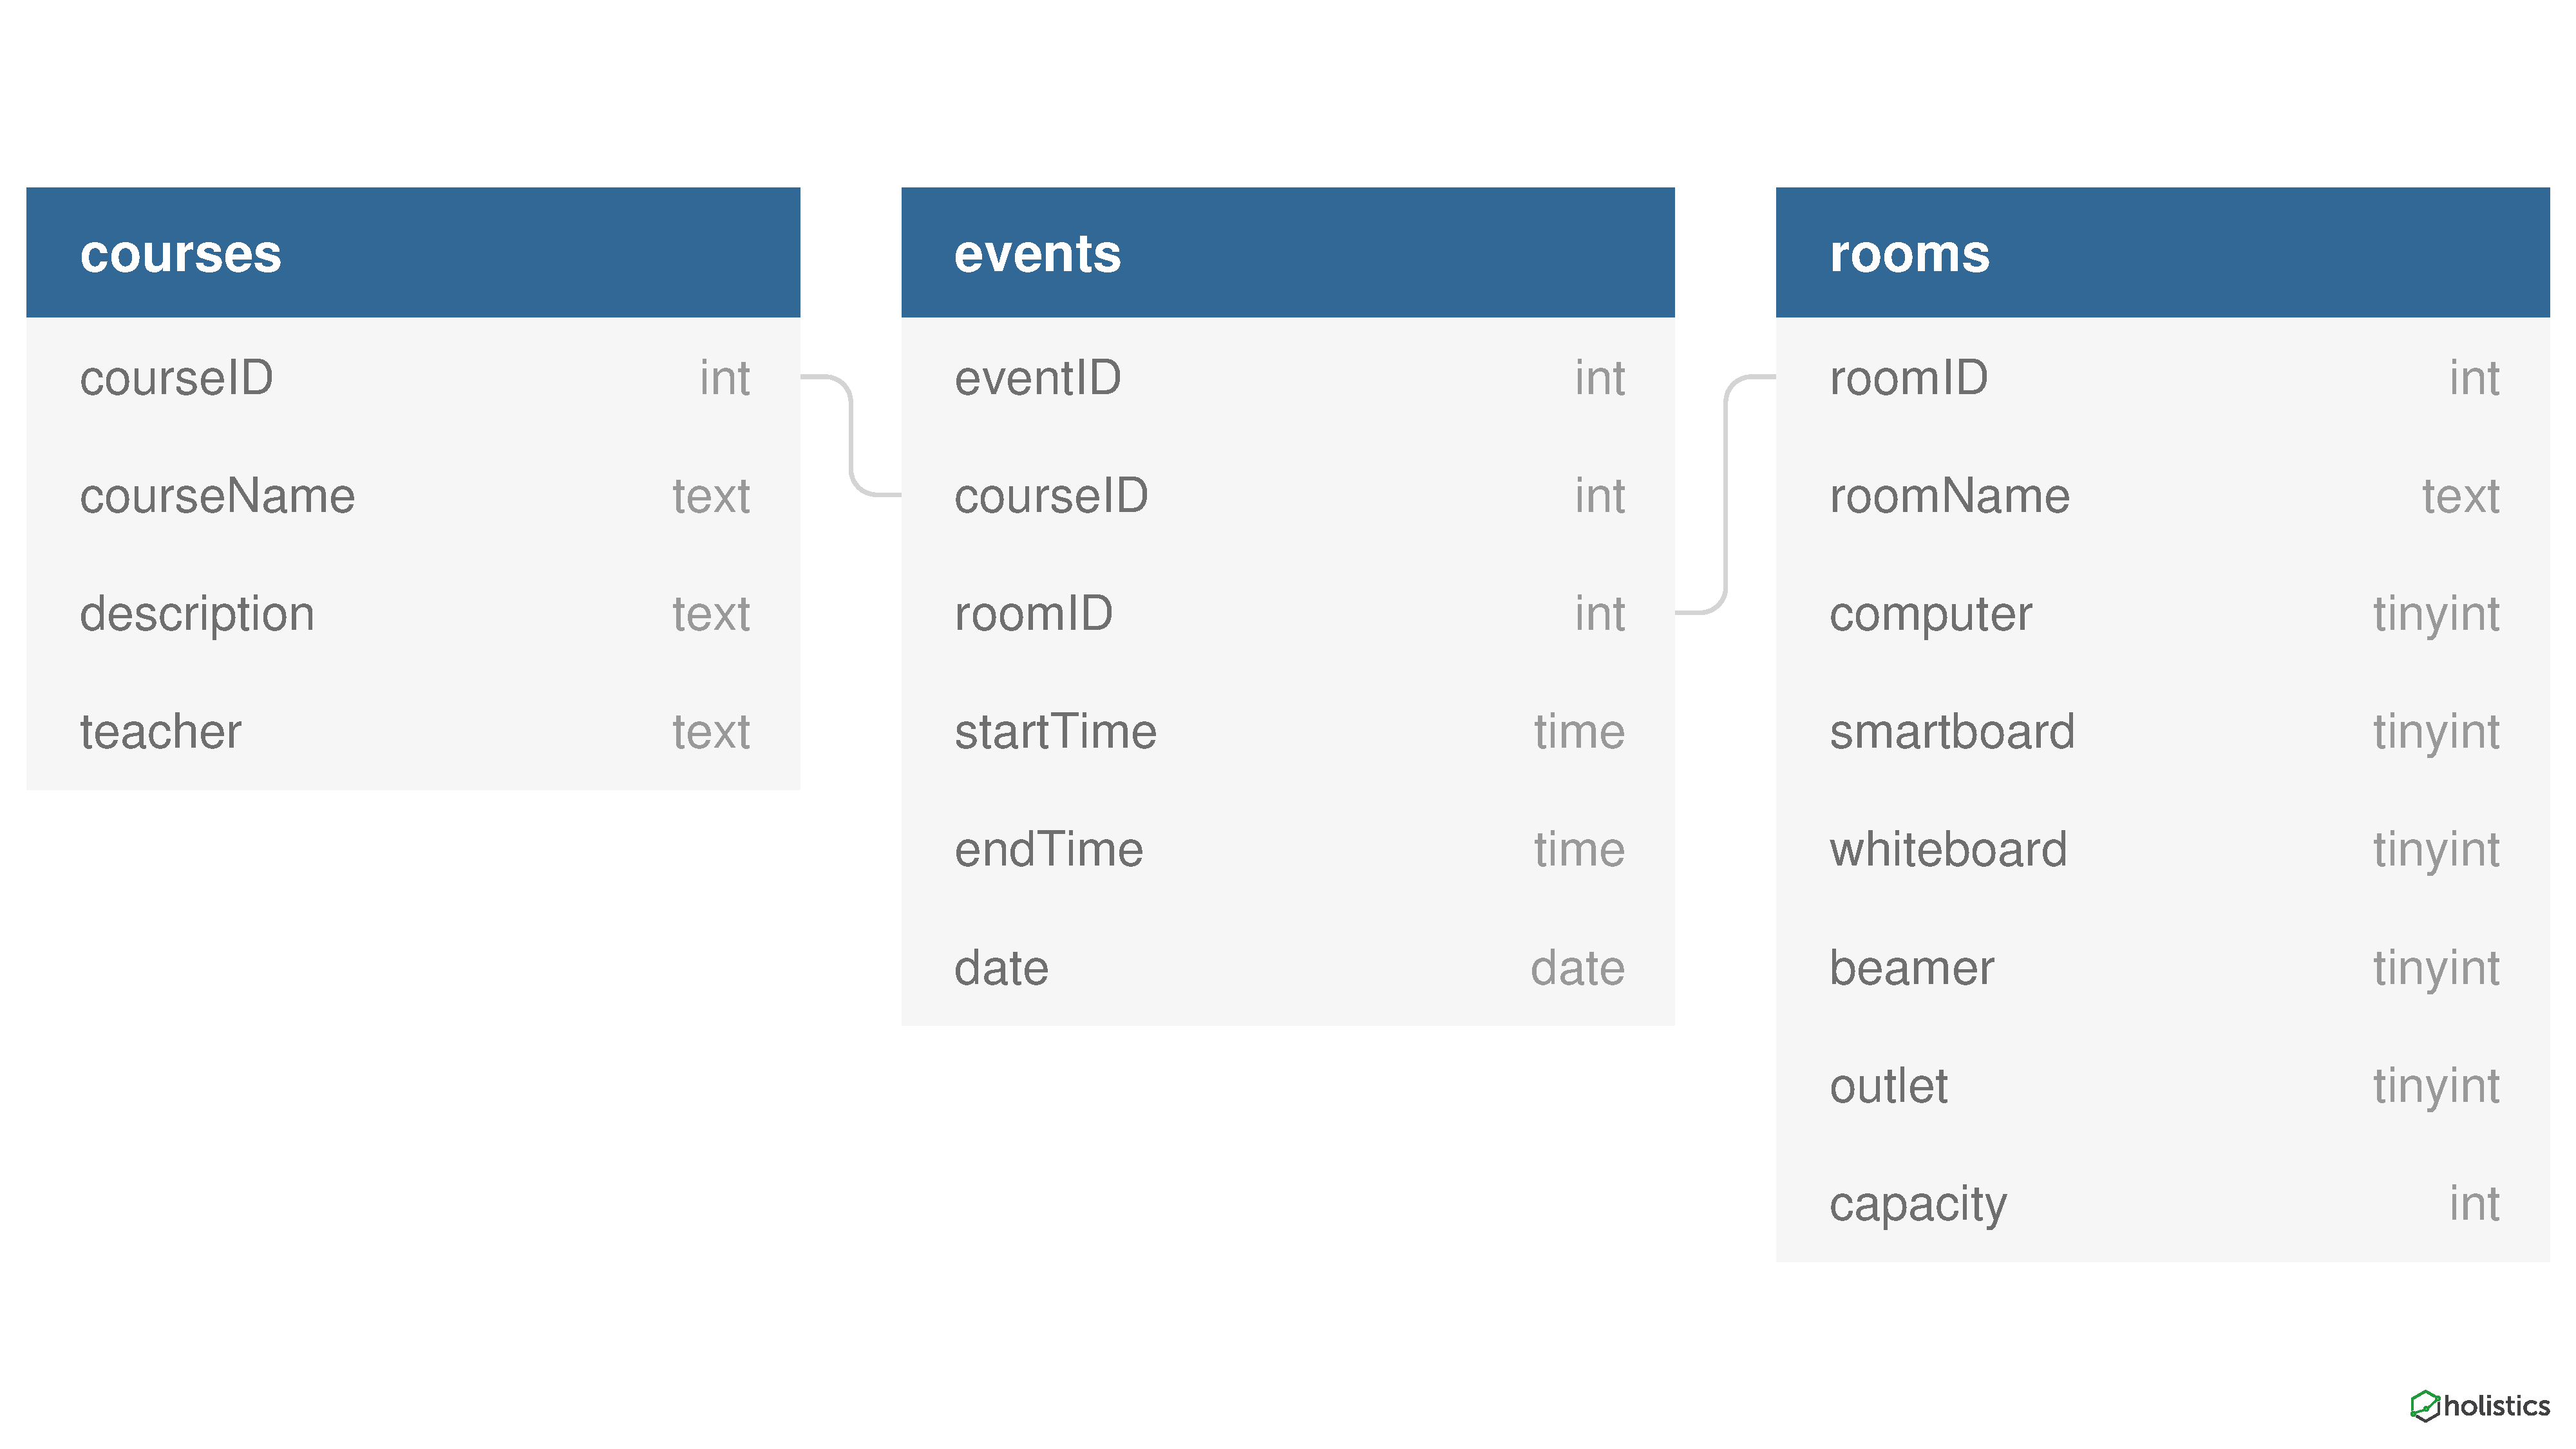
\includegraphics[width=0.9\textwidth]{dbstruct}
	\caption{Database structuur}
	\label{fig:dbstruct}
\end{figure}
\subsubsection{Wifi Access Point op Raspberry Pi}
Voor het opzetten van de WAP op de Raspberry Pi werd een online step-by-step guide gevolgd \cite{RaspberryPiWAP}. De belangrijkste services die hiervoor geïnstalleerd werden op de Raspberry Pi zijn \verb|hostapd| en \verb|dnsmasq|.
\paragraph{DNSmasq} \mbox{}\\ 
Deze service is in principe gewoon een DHCP (Dynamic Host Configuration Protocol) server. Deze zal ervoor zorgen dat een dynamisch IP adres kan toegekend worden op het netwerk zonder dat alle apparaten manueel moeten verbonden worden. In de config file van dnsmasq (die zich onder het volgende path bevindt \verb|/etc/dnsmasq.conf|) wordt een range toegekend van IP adressen die de Wifi kan gebruiken om toe te kennen aan apparaten. Verder wordt ook bepaald hoelang deze IP adressen kunnen gebruikt worden door de apparaten die zich verbinden met het Wifi netwerk. De config file ziet er dan als volgt uit \ref{fig:dnsmasq} .
\begin{figure}[!h]
	\begin{verbatim}
	interface=wlan0
	dhcp-range=192.168.0.11,192.168.0.30,255.255.255.0,24h
	\end{verbatim}
	\caption{dnsmasq.conf}
	\label{fig:dnsmasq}
\end{figure}
\paragraph{Hostapd} \mbox{}\\
Deze service zorgt ervoor dat er een WAP wordt opgezet. In de config file van hostapd (die zich onder het volgende path bevindt \verb|/etc/hostapd/hostapd.conf|) wordt het SSID en het wachtwoord ingesteld van de WAP. Verder wordt hier ook een bridge ingesteld tussen de ethernet verbinding en de wlan0 van de Raspberry Pi. Dit zorgt ervoor dat er zowel via ethernet als via de WAP toegang kan verkregen worden tot de webserver. Dankzij deze file gebruikt de Wifi steeds channel 7. Ook wordt de Wifi Protected Access (WPA) versie ingesteld en de vorm van management die gebruikt zal worden voor het WPA wachtwoord wordt bepaald. Voor deze opdracht wordt WPA-PSK gebruikt wat staat voor Pre-Shared Key. Een wachtwoord bestaat uit minimaal 8 en maximaal 63 tekens. De config file ziet er dan als volgt uit \ref{fig:hostapd} .
\begin{figure}[!h]
	\begin{verbatim}
	interface=wlan0
	driver=nl80211
	bridge=br0
	hw_mode=g
	channel=7
	wmm_enabled=0
	macaddr_acl=0
	auth_algs=1
	ignore_broadcast_ssid=0
	wpa=2
	wpa_key_mgmt=WPA-PSK
	wpa_pairwise=TKIP
	wpa_pairwise=CCMP
	ssid=teamzoepertoff
	wpa_passphrase=stijnkanniks
	\end{verbatim}
	\caption{hostapd.conf}
	\label{fig:hostapd}
\end{figure}
\newpage
\subsubsection{Webserver en GET request}
De webserver die op de Raspberry Pi draait is een apache 2.4 server die de mogelijkheid heeft om samen te werken met de SQL database. Voor deze specifieke applicatie worden slechts vier van de zes aanwezige files gebruikt:
\begin{itemize}
	\item \verb|dbConnect.php|
	\item \verb|event.php|
	\item \verb|room.php|
	\item \verb|roominfo.php|
\end{itemize}
De overige twee files (\verb|index.php| en \verb|showTable.php|) kunnen nodig zijn indien er via een webbrowser toegang verkregen moet worden tot de lokaalbezetting. Wanneer er een  GET request verstuurd wordt vanuit de MBED, wordt de \verb|index.php| file overgeslagen. Een GET request ziet er als volgt uit: \\ \verb|http://ip-address/E-ink-room/roominfo.php?roomName=02.85|. \\ Er wordt dus rechtstreeks naar \verb|roominfo.php| gegaan en als variabele wordt het nummer meegegeven van het lokaal waarvan de info verkregen moet worden.  De inhoud van \verb|dbConnect.php| werd hierboven al besproken, dus zal hier niet meer verder op ingaan worden. \verb|event.php| en \verb|room.php|, zijn hele kleine files die beide \'{e}\'{e}n enkele klasse bevatten. De UML diagramma's voor deze klassen staan in figuur \ref{fig:uml}.
\begin{figure}[h]
	\centering
	\begin{subfigure}{0.45\textwidth}
		\centering
		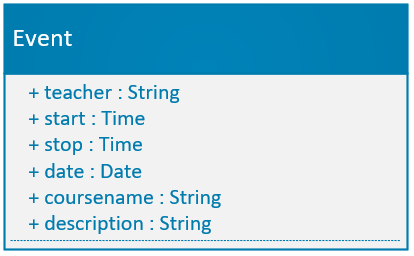
\includegraphics[width=0.95\textwidth]{EventUML.png}
	\end{subfigure}
	\begin{subfigure}{0.45\textwidth}
		\centering
		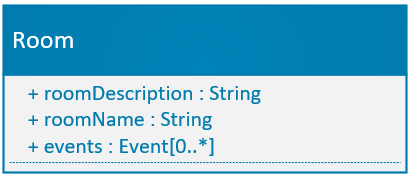
\includegraphics[width=0.95\textwidth]{RoomUML.png}
	\end{subfigure}
	\caption{UML diagram}
	\label{fig:uml}
\end{figure} \\
De laatste en tevens ook grootste file is \verb|roominfo.php|. Hierin worden de klassen die in de vorige files gedefinieerd werden gebruikt. Bij het GET-request wordt een variabele meegegeven die \verb|roomName| genaamd is. Deze wordt opgeslagen in een variabele met de naam \verb|$roomName|. Om veiligheidsredenen is het belangrijk om eerst de door de gebruiker meegegeven variabele te sanitizen. Daardoor kan er geen SQL code geïnjecteerd worden die er eventueel voor kan zorgen dat onze database aangepast wordt zonder dat dit de bedoeling is. De methode die hiervoor gebruikt werd is \verb|mysqli_real_escape_string(string $escapestr)|.

De variabele \verb|$roomName| kan nu gebruikt worden om een query uit te voeren naar de database om zo het \verb|roomID| en de \verb|roomDescription| te kunnen verkrijgen van het opgevraagde lokaal. Het opvragen van deze gegevens gebeurt volgens de code in figuur \ref{fig:roomsql}. Eerst wordt een statement aangemaakt via de \verb|prepare()| methode. Hierin wordt de SQL code gezet met de parameters die moeten geselecteerd worden en de voorwaarde die aangeeft welke entries van de database mogen opgehaald worden. De waarde van de variabele waarop geselecteerd wordt, wordt later toegekend met de \verb|bind_param()| methode. De eerste parameter geeft aan dat we selecteren op een variabele van het type String en de tweede parameter is de variabele zelf. Na de \verb|execute()| methode gebruiken we de \verb|bind_result()| methode om de variabelen van de opgehaalde database entry toe te kennen aan de correcte variabelen zodat ze later gebruikt kunnen worden.  Het roomID is nodig omdat op die manier gezocht kan worden in de event table naar alle geplande events die het opgegeven roomID bevatten.

\begin{figure}
	\begin{verbatim}
		$roomName = mysqli_real_escape_string($conn, $_GET['roomName']);
		$stmt = $conn->prepare("SELECT roomID, roomDescription FROM rooms WHERE roomName=?");
		$stmt->bind_param("s", $roomName);
		$stmt->execute();
		$stmt->bind_result($roomID, $roomDescription);
	\end{verbatim}
	\caption{Info over lokaal ophalen uit database}
	\label{fig:roomsql}
\end{figure}
\newpage
Na het ophalen van het roomID wordt een SQL query uitgevoerd om alle entries uit de events table te halen die doorgaan in het opgevraagde lokaal. De resultaten van deze queries worden gerangschikt in arrays, in dezelfde volgorde als in de table. Zo kan men op een eenvoudige manier de verschillende variabelen opvragen door de indexen te gebruiken van de arrays. Alle elementen van een bepaald event bevinden zich namelijk op de plaats in de array met dezelfde index. Als laatste stap dienen via de courseID's de courseNames opgevraagd te worden in de courses table om zo alle nodige info beschikbaar te hebben om terug te sturen naar de MBED.

Eerst dienen alle gegevens opgestuurd te worden voor ze in een JSON-file kunnen. Hiervoor wordt een object aangemaakt van het type Room. Zoals aangetoond in figuur \ref{fig:uml} heeft dit object 4 objecten. Via de \verb|$myJson  = json_encode($room)| kan het object dan omgezet worden naar een JSON variabele die dan teruggestuurd kan worden met het commando \verb|echo "$myJson";|. Deze JSON-file met alle gegevens wordt dan op de MBED verwerkt.

\subsection{Communicatie tussen de mbed en de database}
{\scriptsize Geschreven door Stijn}
\newline

Teneinde het lessenrooster te printen heeft de mbed gegevens nodig van de database. Communicatie tussen de mbed en de database is dus nodig. De mbed heeft de rol van client en vraagt dus die gegevens aan de database, die logischerwijs de rol van server heeft.
\newline

De communicatie gebeurt via wifi. Op de mbed zit een wi-fi module ESP-WROOM-02 Click \cite{ESP-WROOM-02} die in staat is de data te ontvangen en versturen. In het programma dat loopt op de mbed wordt gebruik gemaakt van 2 functies om gegevens te verkrijgen.

\subsubsection{De verbinding}

Hoe wordt deze verbinding tot stand gebracht?

De eerste functie \verb|init()| maakt verbinding met het wifi access point van de database en gaat als volgt te werk: eerst wordt gecontroleerd of de mbed een wi-fi module heeft (dit is in ons geval de ESP-WROOM-02). Daarna probeert de mbed aan te melden bij de raspberry pi met een opgegeven \verb|WIFI_SSID| en het daarbij horende opgegeven \verb|WIFI_PASSWORD|. Deze  kunnen eenvoudig worden aangepast in een \verb|.json| file.

\subsubsection{De gegevens}

Hoe worden de gegevens uit de database verkregen?

De tweede functie \verb|get(IP_ADDRESS, ROOM)| geeft een \verb|JSON_STRING| terug met daarin alle gegevens voor één lokaal. Het \verb|IP address| en \verb|room number| wordt meegegeven met deze functie. Eerst wordt het GET request samengesteld met de gekregen waarden. Daarna wordt een TCPSocket geopend en gekoppeld aan de Wi-Fi interface, waarna een connectie wordt gelegd met de database. Als die connectie er is, wordt het GET request verstuurd naar de database, die daar dan normaal gezien op antwoordt. De mbed leest de data in en slaat ze op in een buffer. Dit is echter nog de ruwe data. De buffer wordt uitgelezen en enkel de nodige gegevens woren opgeslagen in een tweede buffer. Die laatste is een \verb|JSON_STRING| en wordt dus teruggegeven door de functie.

\subsection{JSON parsing}
{\scriptsize Geschreven door Michel}
\newline

Voor het parsen van de ontvangen JSON strings wordt er gebruik gemaakt Samuel Mokrani’s MedJSONValue library. De library biedt de mogelijkheid aan om een string naar een MbedJSONValue object te parsen. Uit het bekomen object kan dan gemakkelijk aan de hand van de JSON keys de warden gehaald worden en derect getypecast worden naar het gedefineerde type. In tegenstelling met vele andere librarys kan deze wel overweg met JSON arrays van objecten, meeste librarys ondersteunen alleen het parsen van single-type arrays. Een handige feature is date r ook makkelijk nagegaan kan worden hoeveel elementen een array bevat. \ref{fig:json}

\begin{figure}[h]
	\centering
	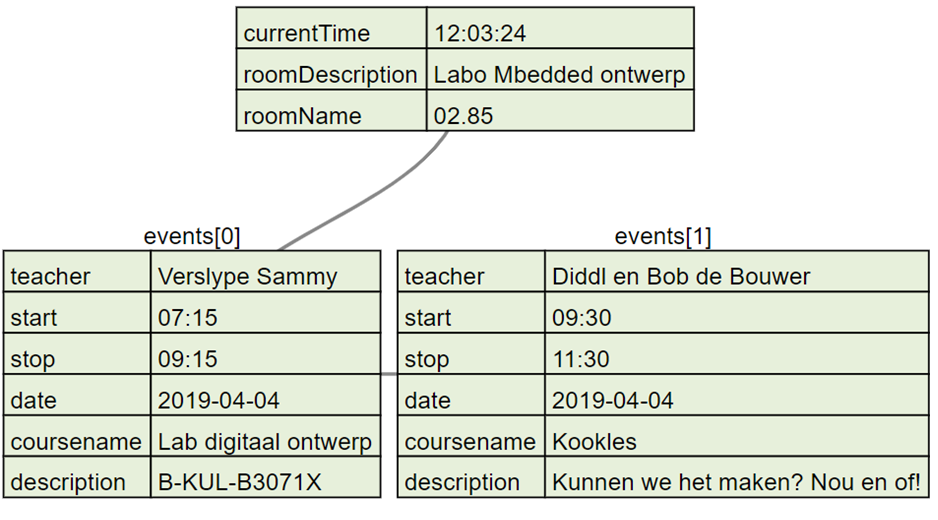
\includegraphics[width=0.75\textwidth]{json}
	\label{fig:json}
	\caption{overzicht van de json parser}
\end{figure}

\subsection{E-paper display}
{\scriptsize Geschreven door Michel}
\newline

De driver is gebaseerd op een arduino library die door de producent van de display beschikbaar gesteld is geweest. Deze werdt geport naar MBED. Aan de hand van een proof of concept art is er besloten hoe het scherm ingedeeldt wordt. Het tekenen van de objecten gebeurt in een lus die telkens een klein deel van het scherm gaat renderen. Dit is zo besloten zodat de beeld buffer variable kan gemaakt worden om RAM gegeugen uit te sparen. Na het renderen van een sub-frame wordt die naar de S-RAM van het beeldscherm geschreven langs de SPI bus. Eenmaal alle sub-frames gerendert en weggeschreven zijn wordt het signal gegeven aan de display om zijn S-RAM te displayen.

\newpage

\section{Resultaten}
{\scriptsize Geschreven door Ine}
\newline

We zijn er in geslaagd om uit de databank info van lokaal 02.85 filteren en in een tabel zetten. Zie figuur \ref{fig:vboutput}.
\newline

\begin{figure}[h]
	\centering
	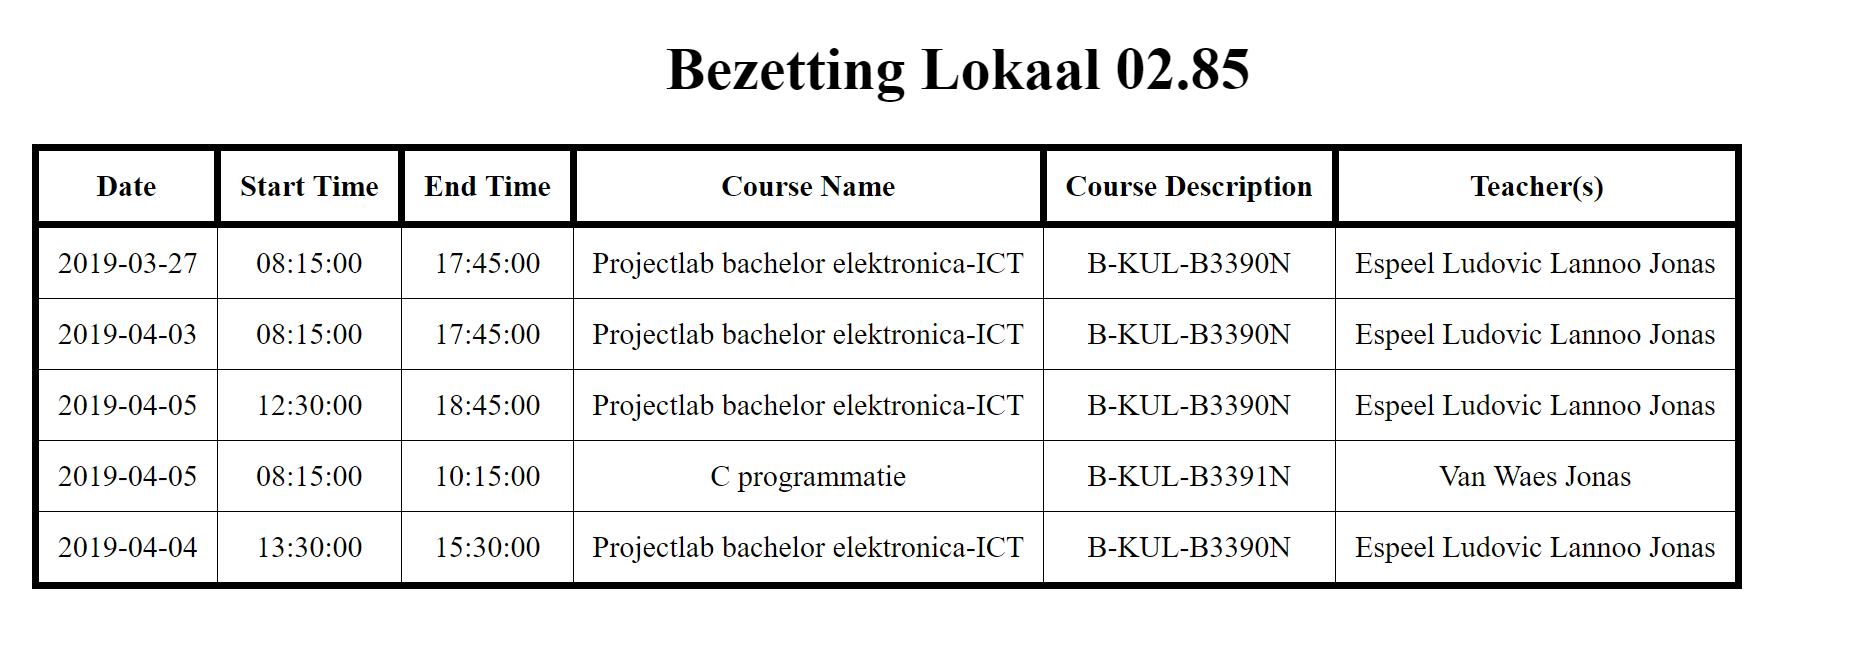
\includegraphics[width=1\textwidth]{vbDatabank}
	\caption{lokaalbezetting lokaal 02.85}
	\label{fig:vboutput}
\end{figure}

Wanneer we merkten dat dit werkte, hebben we daar nog data aan toegevoegd. Ook wordt de data niet meer in een bestand opgeslagen, omdat dit moeilijk is om door te sturen. Nu kunnen we de info van lokaal 02.85 filteren op 4 april 2019. Zie figuur \ref{fig:vbdata}. Alles staat nu als tekst na elkaar. Dit is gemakkelijker om door te sturen. Eens het doorgestuurd is, kunnen we er opnieuw de juiste data uit filteren en er een tabel van maken om op een overzichtelijke manier op de display weer te geven.
\newline

\begin{figure}[h]
	\centering
	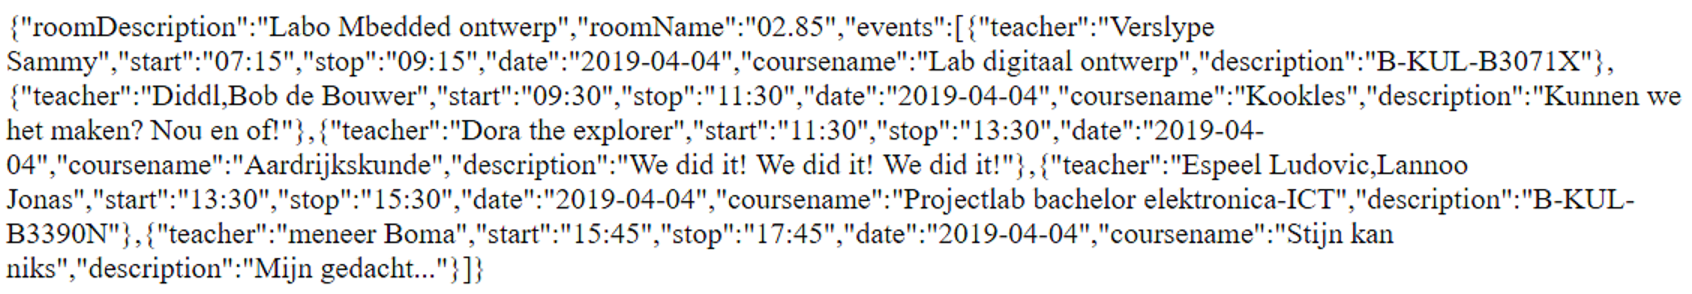
\includegraphics[width=1\textwidth]{vbData02_85}
	\caption{lokaalbezetting lokaal 02.85 op 04/04/2019}
	\label{fig:vbdata}
\end{figure}

We kunnen ook een figuur op de E-ink display afbeelden. Figuur \ref{fig:vbscherm} is een voorbeeld van voor we de data uit de databank konden doorsturen. Hier staan dus nog geen lessen in, maar het toont de lay-out van de display.
\newline
\newline

\begin{figure}[h]
	\centering
	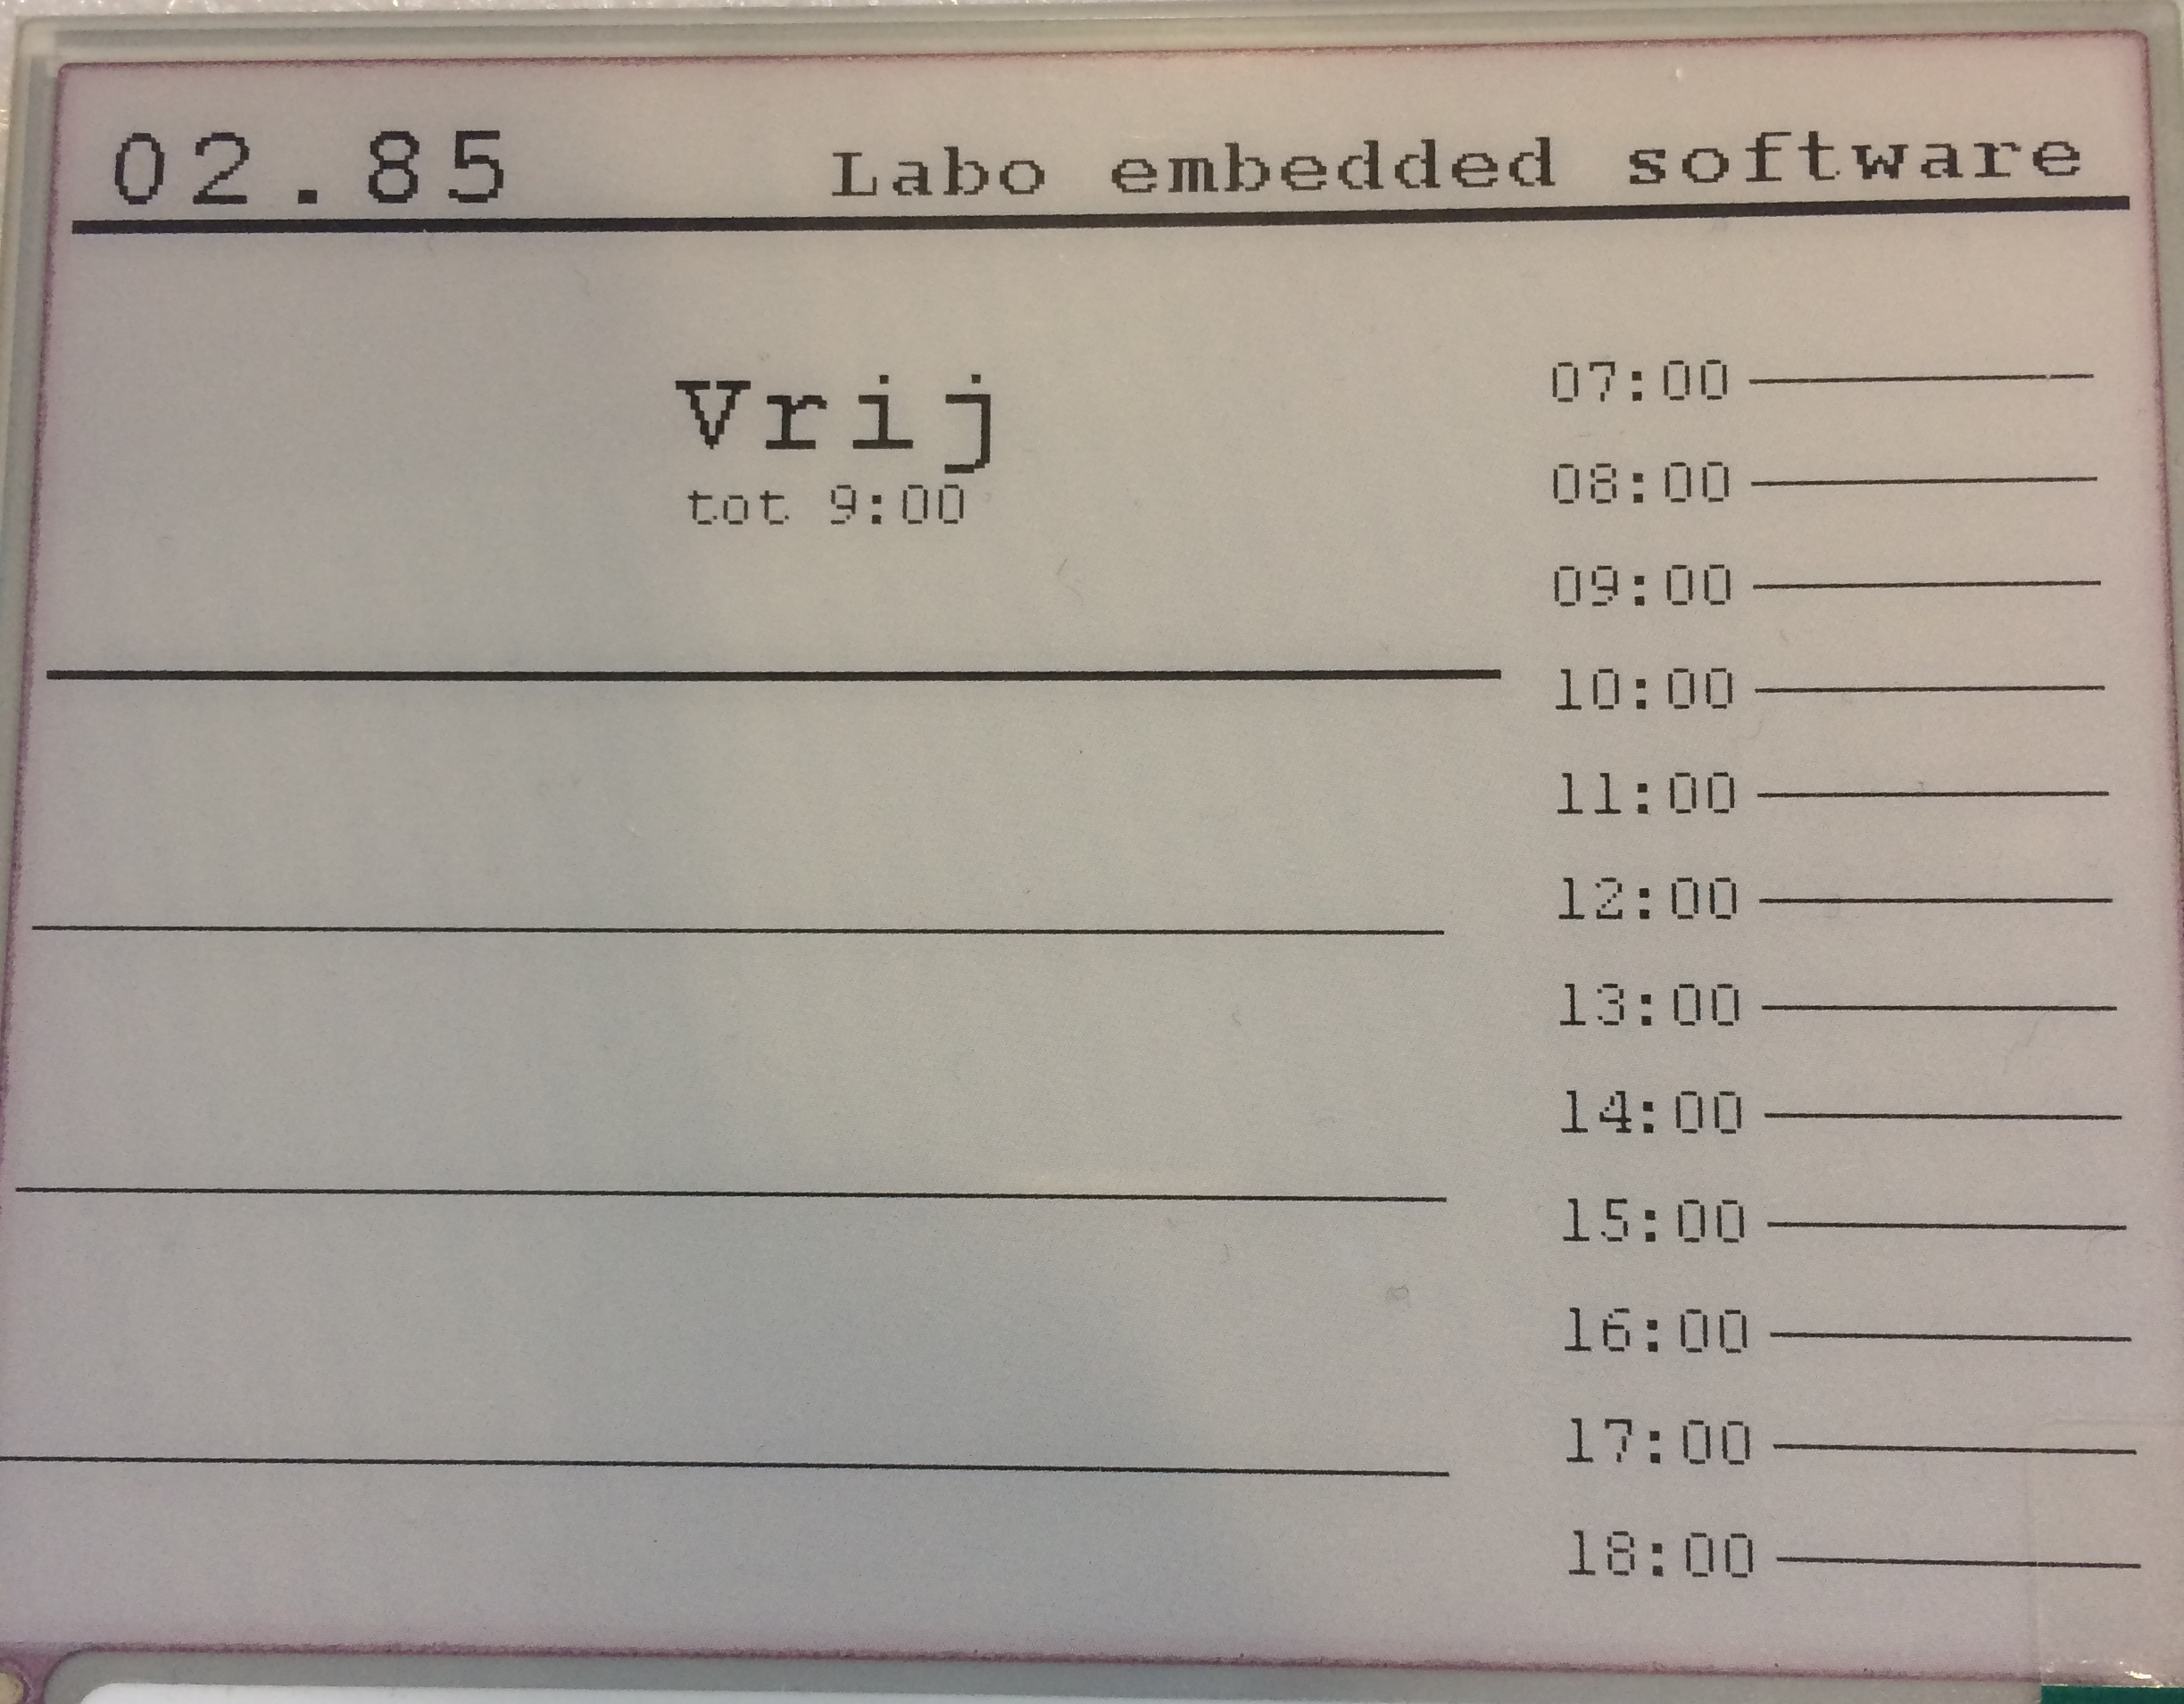
\includegraphics[width=0.75\textwidth]{vbScherm}
	\caption{E-ink display}
	\label{fig:vbscherm}
\end{figure}

De database en het accesspoint waren relatief snel opgezet. Ook iets afbeelden op de display ging relatief vlot. Het moeilijkste was om de data te kunnen versturen naar de display. Het was ook niet eenvoudig om een framebuffer te maken, omdat we dachten dat het niet mogelijk was om een buffer te maken van het hele scherm. We hebben het scherm dus moeten verdelen zodat we voor elk stuk apart een buffer konden maken en zo het scherm stuk per stuk up te daten.
\newline
\newline

Uiteindelijk is in figuur \ref{fig:res} te zien wat het resultaat van dit project is. Links (\ref{fig:concept}) is te zien wat het doel van het project was. Rechts (\ref{fig:result}) is het resultaat te zien wat wij hebben kunnen realiseren.

Hier is te zien dat het gelukt is om de verschillende zaken op het scherm te zetten die we op voorhand bedacht hadden. Op de tijdslijn is met rood aangeduid wanneer het lokaal niet vrij is. In dit voorbeeld is het lokaal dus niet bezet tot 9:30. Daarna zijn wel nog lessen gepland die ook zichtbaar zijn. 

\begin{figure}[h]
	\centering
	\begin{subfigure}{0.45\textwidth}
		\centering
		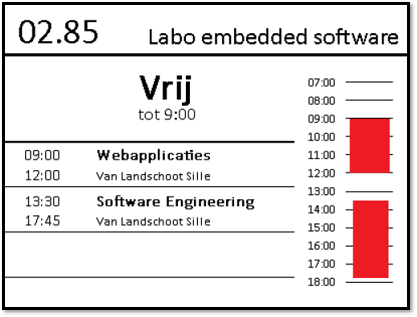
\includegraphics[width=0.95\textwidth]{concept}
		\caption{concept}
		\label{fig:concept}
	\end{subfigure}
	\begin{subfigure}{0.45\textwidth}
		\centering
		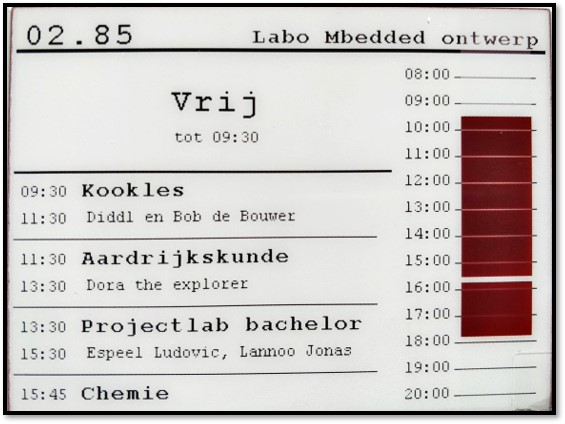
\includegraphics[width=0.95\textwidth]{resultaat}
		\caption{resultaat}
		\label{fig:result}
	\end{subfigure}
	\caption{Het resultaat van dit project}
	\label{fig:res}
\end{figure}

\newpage

\section{In het vervolg}
{\scriptsize Geschreven door Ine}
\newline

Als we dit project verder zouden uitwerken, zouden we een andere mbed en wifi module gebruiken. Nu hebben we veel tijd verloren met het zoeken naar hoe we iets moeten implementeren. We zouden kunnen werken met modules die we kennen, waardoor alles sneller zou kunnen gaan. 
\newline

We hebben veel tijd verloren door te zoeken naar hoe we een framebuffer van heel het scherm kunnen maken. We dachten dat dat niet mogelijk was, dus hebben we een oplossing gezocht om een buffer van een deel van het scherm te maken. Dit was niet gemakkelijk en heeft veel tijd ingenomen. Achteraf hebben we gehoord dat het wel mogelijk is om heel het scherm in één keer up te daten. We zouden dus kunnen uitzoeken hoe dat werkt en het scherm op die manier implementeren, omdat het updaten van het scherm zo sneller zou gaan. 
\newline

Verder zouden we ook tijdens het zoeken naar oplossingen proberen meer geduld te hebben. Als er problemen waren met dingen die we niet begrepen, zouden we moeten efficiënter zoeken naar oplossingen. We zouden kunnen één manier van werken proberen volledig uit te werken en te begrijpen, in plaats van telkens iets kleins niet lukt, een volledig nieuwe manier te zoeken.
\newline

Tijdens het project hebben we ondervonden dat de database elke les een nieuw IP adres kreeg. Dit heeft af en toe voor problemen gezorgd. Het zou dus gemakkelijker zijn als we de database een statisch IP adres zouden geven. 
\newline

Als we nog wat meer tijd hadden gehad, zouden we kunnen zoeken naar een manier om de JSON buffer automatisch af te laten kappen wanneer alle bruikbare data er in zit. Tot nu toe krijgt de buffer een vaste lengte, en de plaats die niet gebruikt wordt, wordt opgevuld met onleesbare tekens. Dit zou dan niet meer gebeuren.

\newpage

\section{Conclusie}
{\scriptsize Geschreven door Ine}
\newline

We hebben een manier gevonden om op een energie zuinige manier een leslokaal dynamisch aan te duiden. We kunnen op een E-ink display aanduiden op welke uren van de dag het lokaal vrij is. Wanneer het lokaal niet vrij is, is duidelijk wie in het lokaal zit, welk vak er op dat moment gegeven wordt en hoe lang het nog zal duren voor het lokaal  weer vrij is.

\newpage

\bibliographystyle{plain}
\bibliography{library}

\end{document}
